\documentclass[../practica_02.tex]{subfiles}

\begin{document}

    \begin{enumerate}
        \item
            \quad $ r(t) = \left\{
                \begin{array}{ll}
                    t(0; -4) + (0; 2) t \in [0,1]\\
                    (t-1)(1; 0) + (0; 2) t \in (1,2)\\
                    (t-2)(1; 0) + (0; -2) t \in [2,3)\\
                    (t-3)(0; -4) + (1; 2) t \in [2,3]\\
                \end{array}
                \right.$

            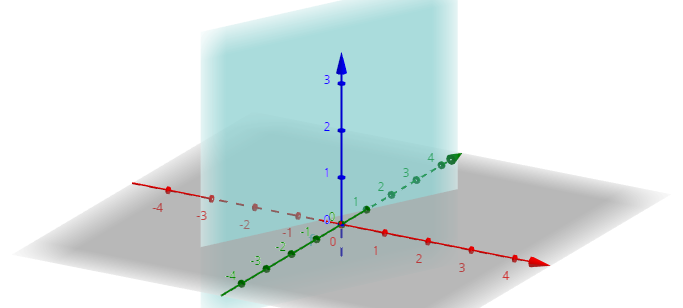
\includegraphics[scale=0.8]{ej11/resources/a.png} $ $

            $ $

        \item 
            \quad $ r(t) = \left\{
                \begin{array}{ll}
                    t(-2; 0) + (1; 0) t \in [0,1]\\
                    (t-1)(1; 1) + (-1; 0) t \in (1,2)\\
                    (t-2)(1; -1) + (0; 1) t \in [2,3]\\
                \end{array}
                \right.$

            $ $

            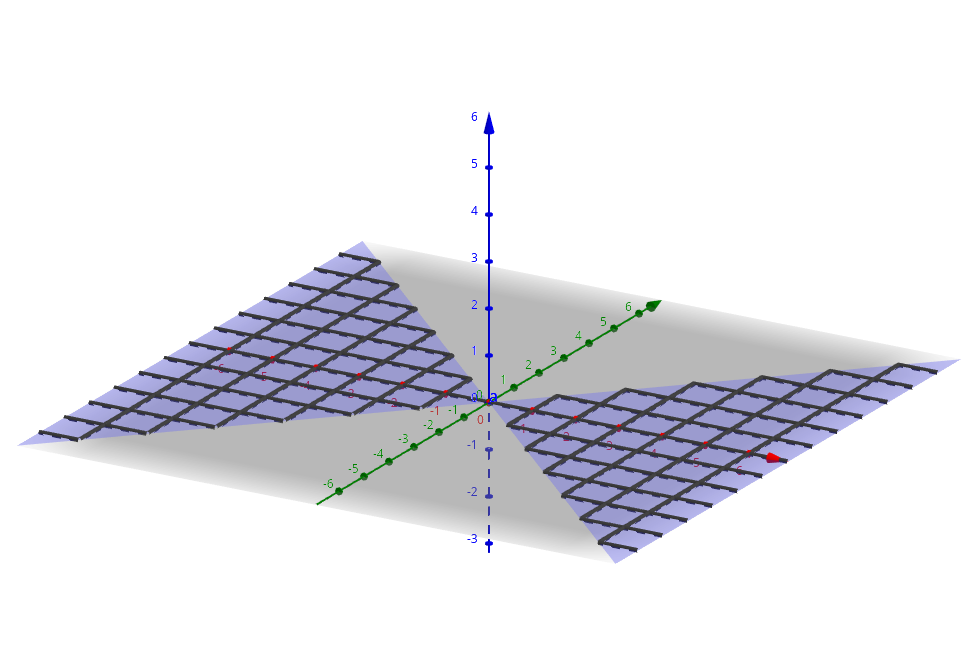
\includegraphics[scale=1]{ej11/resources/b.png} $ $

    \end{enumerate}

\end{document}